\documentclass[11pt]{beamer}
\usetheme{Copenhagen}
\usepackage[utf8]{inputenc}
\usepackage[spanish]{babel}
\usepackage{amsmath}
\usepackage{amsfonts}
\usepackage{amssymb}
\usepackage{graphicx}
\author{Onofre Martorell, Lidia Talavera}
\title{Image segmentation}
%\setbeamercovered{transparent} 
%\setbeamertemplate{navigation symbols}{} 
%\logo{} 
%\institute{} 
%\date{} 
%\subject{} 
\begin{document}

\begin{frame}
\titlepage
\end{frame}

%\begin{frame}
%\tableofcontents
%\end{frame}

\begin{frame}{Introduction}

\begin{block}{Goal}
We want to segment an image $f$ through the Chan-Vese Segmentation.
\end{block}
An example of image to segment:
\begin{figure}
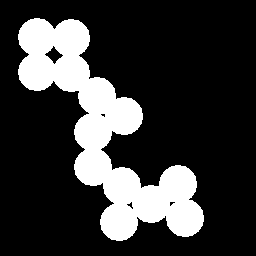
\includegraphics[scale=0.4]{circles}
\end{figure}
\end{frame}

\begin{frame}{Chan-Vese segmentation}
The Chan-Vese segmentation finds the curve $C$ that is the boundary of the segmentation. The way to find that curve is minimizing the following functional:
$$\text{arg min}_{c_1,\ c_2,\ C }\ \mu \text{Lenght}(C) +\nu\text{Area}(inside(C)) +$$$$ \lambda_1\int_{inside(C)}|f(x)-c_1|^2dx + \lambda_2\int_{outside(C)}|f(x)-c_2|^2dx,$$
where $C$ is the boundary of a closed set and $c1$, $c2$ are the values of $u$ respectively inside and outside of $C$. 
\end{frame}

\begin{frame}{Level set functions}
As it is difficult to manipulate $C$ we will use a function $\phi$ and the $C$ will be the zero crossing of $\phi$ that is 
$$C = \{x\in \Omega:\phi(x) = 0\}.$$
With this the functional is rewritten as:

$$\text{arg min}_{c_1, c_2, \phi}\ \mu \int_{\Omega}\delta(\phi(x))|\nabla\phi(x)|dx+\nu \int_{\Omega}H(\phi(x))dx +$$$$ \lambda_1\int_{\Omega}|f(x)-c_1|^2H(\phi(x))dx + \lambda_2\int_{\Omega}|f(x) -c_2|^2(1-H(\phi(x)))dx,$$
\end{frame}
\begin{frame}{Level set functions}
In the previous formula $H$ denotes the Heaviside function and $\delta$ the Dirac mass, its distributional derivative:
$$ H = \left\lbrace\begin{array}{l l}
1&t\geq 0,\\
0 & t<0
\end{array}\right. ,\quad \delta(t) = \frac{d}{dt}H(t).$$

Note that we cannot derive $H(t)$. Because of that, in the implementation we take the Heaviside function as
$$H_{\epsilon}(t) = \frac{1}{2}\bigg(1 + \frac{2}{\pi}\arctan \bigg(\frac{t}{\epsilon}\bigg)\bigg)$$
and the Dirac mass as
$$\delta_{\epsilon} = \frac{\epsilon}{\pi(\epsilon^2)+t^2)}$$
\end{frame}



\begin{frame}{Implementation}
Now we have to minimize the functional respect to $c_1$, $c_2$ and $\phi$.

The way to do it is the following:
\begin{enumerate}
\item Update $c_1$ and $c_2$ as $$c_1 =  \text{ and } c_2 = $$.
\item Evolve $\phi$ using the semi-implicit gradient descent $$\phi_{i,j} = $$. 
\end{enumerate}
\end{frame}

\begin{frame}{Results}

\end{frame}

\end{document}